\section{Background}
\subsection{Frequency Components}
Consider a simple sinusoid with the frequency $\omega_0$ representing, for example, displacement $u$ as a function of time $t$,
\begin{gather}
u\left(t\right)=\sin\left(\omega_0t\right),
\end{gather}
with little effort, its time derivatives can be derived as
\begin{gather}
v\left(t\right)=\ddfrac{u\left(t\right)}{t}=\omega_0\cos\left(\omega_0t\right),\qquad
a\left(t\right)=\ddfrac{v\left(t\right)}{t}=-\omega_0^2\sin\left(\omega_0t\right).
\end{gather}
It is evident that the magnitudes of velocity $v$ and acceleration $a$ are scaled by $\omega_0$ and $\omega_0^2$, respectively. Now consider an arbitrary integrable function of time representing, again, displacement $u$. Its Fourier transform can be expressed as
\begin{gather}
\hat{u}\left(\omega\right)=\int_{-\infty}^{\infty}u\left(t\right)\exp\left(-i\omega{}t\right)\md{t}.
\end{gather}
Accordingly, for $v$ and $a$, one can obtain
\begin{gather}\label{eq:scaling}
\begin{split}
\hat{v}\left(\omega\right)=i\omega\hat{u}\left(\omega\right),\qquad
\hat{a}\left(\omega\right)=i\omega\hat{v}\left(\omega\right)=\omega^2\hat{u}\left(\omega\right).
\end{split}
\end{gather}
If the energy spectrum of $\hat{u}\left(\omega\right)$ is known, then the corresponding spectra of $\hat{v}\left(\omega\right)$ and $\hat{a}\left(\omega\right)$ can be computed by multiplying $\hat{u}\left(\omega\right)$ by $\omega$ and $\omega^2$, respectively. The simple sinusoid example is a slice of the spectra at $\omega=\omega_0$.

The above expressions indicate that if the original $u\left(t\right)$ contains some high frequency components (at some $\omega=\omega_h$), although with potentially relative small magnitude compared with low frequency components (at some $\omega=\omega_l$), i.e., $\norm{\hat{u}\left(\omega_h\right)}^2\ll\norm{\hat{u}\left(\omega_l\right)}^2$, the corresponding $\norm{\hat{v}\left(\omega_h\right)}^2$ and $\norm{\hat{a}\left(\omega_h\right)}^2$ may not be small, since they are scaled by $\omega_h$ and $\omega_h^2$.
\subsection{External Loads}
In the context of the finite element response history analysis, seismic action can be introduced into the system via either force or deformation. For the former, acceleration record is converted to inertial force with the assist of mass and then applied to target degrees of freedom. For the latter, displacement record can be directly applied to supports to shake the structure as if it sits on a shaking table.
The typical sampling rate of ground motion seismograms ranges from \SI{50}{\hertz} to \SI{200}{\hertz}. This corresponds to a sampling period $T_s$ from \SI{5}{\milli\second} to \SI{20}{\milli\second}. Often such a time step size is not sufficient for non-linear response history analysis due to convergence issues. Ideally, the continuous--time version needs to be reconstructed from the discrete--time version of input seismogram in order to allow a smaller time step size to be used for simulation. However, it is obvious that the exact reconstruction is not achievable.

It is then a convention to perform linear interpolation between two adjacent discrete samples for the case that time step size (of numerical analysis) is different from sampling interval (of input seismogram). Essentially, the linear interpolation is equivalent to a low--pass finite impulse response (FIR) filter with a triangular window.

For the ease of discussion, let sampling interval be the multiple of time step size and let the ratio be $L$, which is an integer. It is then equivalent to upsample the input seismogram by the same ratio $L$. If the sampling rate/frequency of the original seismogram is $\omega_s$, then the upsampled signal has a sampling rate of $L\omega_s$. Extra attention shall be paid to the original Nyquist frequency $\omega_s/2$ since anything above it cannot be reconstructed. For a discrete--time signal $u[n]$, a typical upsampling operation with upsampling factor $L$ consists of two steps:
\begin{enumerate}
\item Insert $L-1$ zeros between each pair of adjacent samples in $u[n]$, resulting in a new signal $u_e[n]$ which can be formally defined as
\begin{gather}
u_e[n]=\left\{
\begin{array}{ll}
u[n/L],&n=0,L,2L,3L,\cdots,\\
0,&\text{otherwise}.
\end{array}
\right.
\end{gather}
This is called an expander, and is often denoted by $\uparrow{}L$ such that $u_e[n]=[\uparrow{}L]u[n]$.
\item Apply a low--pass filter with kernel $h[n]$ on $u_e[n]$ via convolution. The linear interpolation corresponds to the following kernel.
\begin{gather}
h[n]=\left\{
\begin{array}{ll}
1-\abs{n}/L,&\abs{n}\leqslant{}L-1,\\
0,&\text{otherwise}.
\end{array}
\right.
\end{gather}
The interpolated/filtered signal is denoted as $u_i[n]$. In this work, different kernels will be discussed.
\end{enumerate}
\subsection{Oscillator}
Consider a simple mass--spring--dashpot linear oscillator system subject to external load $p\left(t\right)$ with the following equation of motion
\begin{gather}
ma\left(t\right)+cv\left(t\right)+ku\left(t\right)=p\left(t\right),
\end{gather}
Duhamel's integral shows the solution to this system can be expressed as
\begin{gather}\label{eq:duhamel}
u\left(t\right)=\int_{0}^{t}p\left(\tau\right)h\left(t-\tau\right)\md{\tau},
\end{gather}
with the fundamental solution
\begin{gather}
h\left(t\right)=\dfrac{1}{m\omega_d}\exp\left(-\zeta\omega_nt\right)\sin\left(\omega_dt\right)
\end{gather}
where $m$ is the mass, $c$ is the damping coefficient, $k$ is the stiffness, $\omega=\sqrt{\dfrac{k}{m}}$ is the natural frequency of the system, $\zeta=\dfrac{c}{2\sqrt{mk}}$ is the damping ratio, $\omega_d=\omega_n\sqrt{1-\zeta^2}$ is the dampened frequency. \eqsref{eq:duhamel} is essentially the convolution of two functions $p\left(t\right)$ and $h\left(t\right)$ such that
\begin{gather}
u\left(t\right)=\left(p\ast{}h\right)\left(t\right)=\left(h\ast{}p\right)\left(t\right),
\end{gather}
since convolution is commutative.

If the external load $p\left(t\right)$ is treated as a signal and the fundamental solution $h\left(t\right)$ is treated as a filter kernel, the discrete--time solution $u[t]$ can be approximated by
\begin{gather}
u[t]=\left(p\ast{}h\right)[t].
\end{gather}
with the sampled $p[t]$ and $h[t]$. The discrete--time kernel $h[t]$, which represents a dampened low--pass filter, can be obtained by truncating $h\left(t\right)$ following a similar procedure used in the window design method. The maximum gain is achieved at $\omega=\omega_d$ and high frequency components of $p[t]$ are attenuated by $h[t]$.
\section{A Close Look}
Since the extended discrete signal $u_e[n]$ is $u[n]$ with additional zero samples, once the upsampling factor $L$ is chosen, $u_[n]$ can be converted to $u_e[n]$ and vice versa. We focus on the properties of $u_e[n]$.

The bare $u_e[n]$ without any filters contains spectral images, that is, extra copies of the original spectrum $\omega\in[0,~\omega_s/2]$ in additional frequency domain $\omega\in[\omega_s/2,~L\omega_s/2]$.
\begin{figure}[ht]
\centering
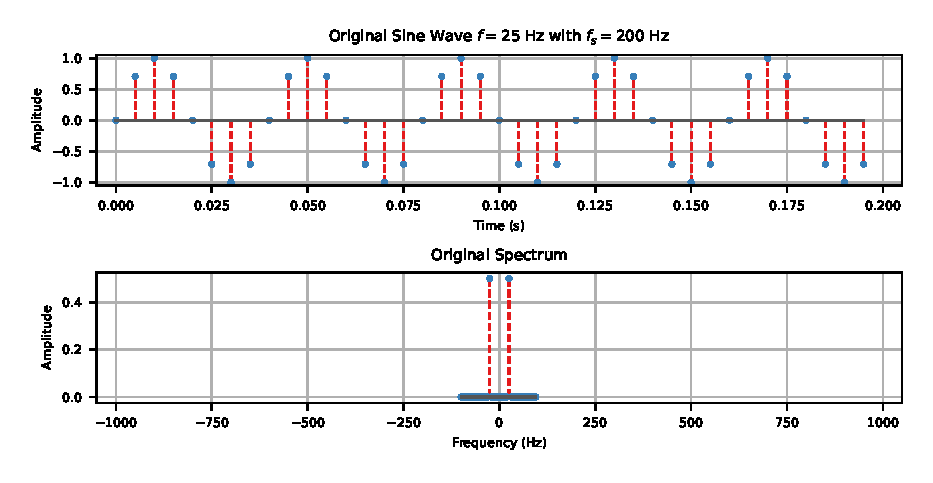
\includegraphics{PIC/PureSineOrigin}
\caption{original sine wave in time domain and frequency domain}\label{fig:original}
\end{figure}
Consider the sinusoid
\begin{gather}
u(t)=\sin\left(2\pi{}f_0t\right),
\end{gather}
with the frequency $f_0=\dfrac{\omega_0}{2\pi}$ chosen to be \SI{25}{\hertz}. Assume this continuous--time signal is sampled at rate $f_s=\SI{200}{\hertz}$, the discrete--time signal $u[n]$ can be depicted in \figref{fig:original}. The corresponding Nyquist frequency is $f_s/2=\SI{100}{\hertz}$, thus, the frequency ranges from \SI{-100}{\hertz} to \SI{100}{\hertz}.

By choosing an upsampling factor $L=10$, the extended signal $u_e[n]$ (zero--stuffed) can be illustrated as in \figref{fig:extended}. The Nyquist frequency of $u_e[n]$ is $10\times\SI{100}{\hertz}=\SI{1000}{\hertz}$, the original component at $\SI{25}{\hertz}$ is copied in the additional frequency domain ranging from \SI{100}{\hertz} to \SI{1000}{\hertz} (negative frequency as well).
\begin{figure}[ht]
\centering
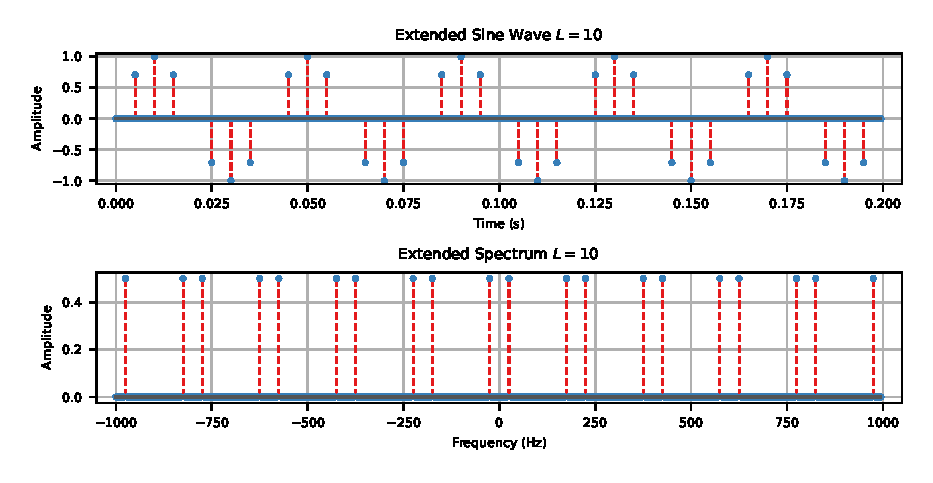
\includegraphics{PIC/PureSineExtended}
\caption{zero--stuffed sine wave in time domain and frequency domain}\label{fig:extended}
\end{figure}

The linear interpolation (triangular window) can be constructed as
\begin{gather}
h[n]=\begin{bmatrix}
1&2&3&\cdots&10&\cdots&3&2&1
\end{bmatrix},
\end{gather}
its frequency response can be seen in \figref{fig:tri_window}.
\begin{figure}[ht]
\centering
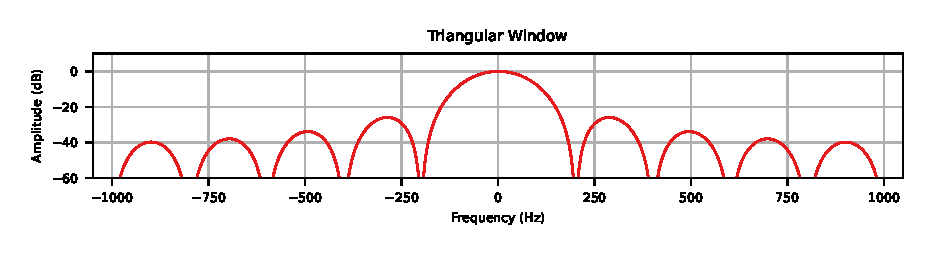
\includegraphics{PIC/TriangularWindow}
\caption{triangular window in frequency domain}\label{fig:tri_window}
\end{figure}

The upsampled signal can be obtained by either performing the convolution in time domain or multiplication in frequency domain.
\begin{figure}[ht]
\centering
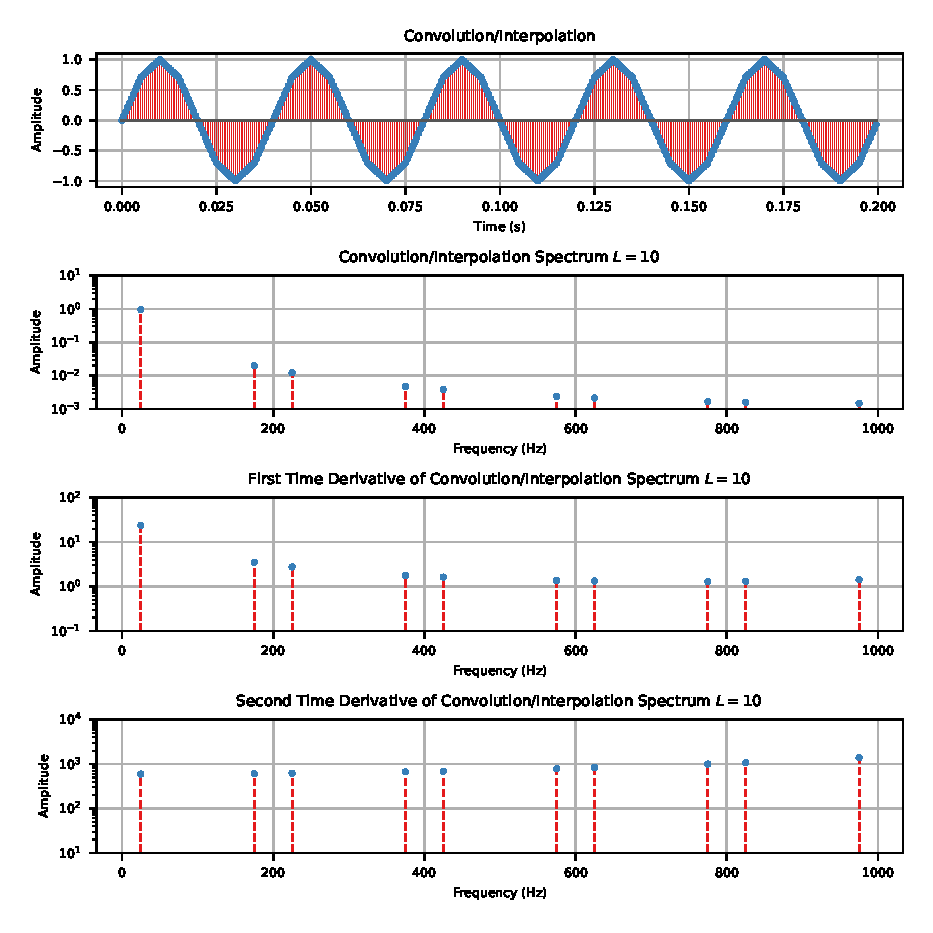
\includegraphics{PIC/Convolution}
\caption{interpolated sine wave and its derivatives in time domain and frequency domain}\label{fig:interpolated}
\end{figure}
\figref{fig:interpolated} shows the interpolated signal and its derivatives in both time domain and frequency domain. Due to the high side lobe level (around \SI{-26}{\decibel} of the first side lobe) of the triangular window, although the spectral images in $u_i[n]$ between \SI{100}{\hertz} and \SI{1000}{\hertz} are seemingly attenuated, the corresponding components in $v_i[n]$ and $a_i[n]$ may have significant magnitudes compared to that of the main lobe.